\documentclass[doc,12pt]{apa}        % use: 'man' for submission type; 'jou' for
                                % journal type, and 'doc' for typical latex
                                % but with figures inline with text
\usepackage{geometry} 
%\geometry{a4paper} 
\usepackage[parfill]{parskip}   % paragraphs delimited by an empty line

\usepackage{graphicx} 
\usepackage{amssymb}            % no idea what this does...
\usepackage{epstopdf}           % no idea what this does...
%\usepackage{gensymb}            % no idea what this does...

\usepackage{setspace}

\DeclareGraphicsRule{.tif}{png}{.png}{`convert #1 `dirname #1`/`basename #1 .tif`.png} \setcounter{secnumdepth}{0}  % no idea what this does...

\usepackage{apacite}
\usepackage{longtable}
%%%%%%%%% END HEADER %%%%%%%%%

\title{Rewards are categories.} 
\author{Erik J. Peterson} \affiliation{Dept. of Psychology \\ Colorado State University \\ Fort Collins, CO} 

%%%%%%%%%%%%%%%%
\begin{document} 
%%%%%%%%%%%%%%%%
\maketitle
\doublespacing

\section{Chapter 3 -- fMRI analyses} % (fold)
\label{sec:task_and_models}
\subsection{An acquisition}
\label{sub:acquired}
\subsubsection{Data Details}
\label{subsub:datadetails}
fMRI data was acquired at the Intermountain Neuroimaging Consortium (INC) facility located at the University of Colorado at Boulder on a Siemens Allegra 3T (whole body) scanner.  All 18 right-handed participants were pre-screened for the typical fMRI exclusion factors (e.g. metal implants, mental disorders, etc).  High resolution anatomical data were acquired as a T1-weighted structural image, MPRAGE sequence, at 1x1x1 mm, (256x156x192) with a TR of 2530 ms, and TE of 1.64 ms, with a flip angle of 7$^\circ$.  All functional (i.e. BOLD) data was acquired with T2-weighted echo-planar imaging (EPI), at 2.29 x 2.29 x 4.00 mm (96 x 96 x 26), with a TR of 1500 ms, a TE a 25 ms, a flip angle of 75$^\circ$ and a FOV of 220 mm.

A total of 4 sets of functional data were acquired.  The first was of the ``refresher'' for part 1 of the behavioral training (p\pageref{subsub:whatwhen}), spanning 241 volumes.  The second and third covered part 2 of the stimulus-responses learning task (again see p\pageref{subsub:whatwhen}), which was divided up into 2 (nearly) even sets so that participants need not be active for more the 10 or so minutes.  Thes sets lasted 390 and 394 volumes respectively.  The fourth acquisition covered a scan, that featured repeated examples from both reward categories in a random order.  The intent of this scan was to isolate rewarding activity outside the primary task. This localizer was not in the end useful (see p\pageref{subsub:chunks}).

\subsubsection{Preprocessed (model) food}
\label{subsub:preprocessed}
Following DICOM to nifiti-1 conversion using dicom2nii (\url{http://www.mccauslandcenter.sc.edu/mricro/mricron/dcm2nii.html}), each dataset was subjected to the following preprocessing pipeline carried out in SPM8's batch mode (\url{http://www.fil.ion.ucl.ac.uk/spm/software/spm8/}).  For complete code see, \url{https://github.com/andsoandso/fmri/tree/master/catreward/spm\_m}.  Anatomical data was first segmented into white and grey matter regions \cite{Collignon:1995p9347}.  Based on these segments, the parameters necessary for normalization into T1 MNI-352 (1 $mm$) space were calculated. Normalization has two steps.  The first is a Bayesian 12-parameter affine transformation \cite{Ashburner:1997p9348}.  The second is a set of nonlinear deformations, using a 1127 parameter discrete cosine transform \cite{Ashburner:1999p9350}.  Anatomical data was then resampled from 1.27 to 1.00 $mm^3$ using fourth degree $\beta$-splines and finally, using the parameters above, normalized into MNI space.

First movement regressors for all volumes of the functional data were calculated \cite{Ashburner:1999p9350}.  No participant moved more than 1.5 $mm$.  Functional data was then slice-time corrected, using slice 13 (the middle slice from the descending acquisition) as the reference, followed by co-registeration with the pre-processed (native-space) anatomical data, and resampling into 3 $mm^3$ voxels again using fourth degree $\beta$-splines \cite{Collignon:1995p9347}.  Functional data was then normalized into MNI space using the anatomically-derived parameters above.  Finally, the functional data was spatially smoothed using a 6 $mm$ FWHM Gaussian, though a copy of the unsmoothed data was retained for the ROI analyses (described on p\pageref{sub:regoins}).  Each voxel's time course was also low-pass filtered using finite impulse response model, with a cutoff at 0.008 Hz, prior to regression analysis \cite{Kruggel:1999p9351}.  For all whole-brain analyses, the movement regressors were entered into as covariates thus accounting for any head movement.  Given the large spatial averages needed for the ROI analyses these analyses weren't motion corrected.

\subsubsection{The best of all possible signals}
\label{subsub:bestsignal}
In fMRI (and in time-series analysis in general) there is an intrinsic trade-off between detecting a signal in the presence of noise and estimating the timecourse (i.e. shape) of that signal \cite{Dale:1999p7901,Birn:2002p1777,Liu:2004p2141}.   One way to optimize over both these objectives is to manipulate the trial order, inside a rapid event-related design \cite{Miezin:2000p7924}.  One state-of-the-art method for optimizing the trial order is a genetic algorithm which uses two (weighted) loss functions, one for signal detection and one for time-course estimation \cite{Wager:2003p2980}. \citeNP{Kao:2009p7899}, improved on Wager's design, adding in psychological considerations, and greatly improving executation speed and documentation.  As a result, Kao \emph{et al's} (2009) method was used to optimize trial orders for part 1 and 2, along with the reward category (i.e. grating only) localizer scan.

\subsection{Mobs of blobs}
\label{sub:blob}
All statistical parametric maps (below) were derived from a Random Effects analysis (RFX, or ``second-level'' in SPM8 jargon), multiple comparison corrected assuming Gaussian Random Fields using the Family Wise Error Rate (FWE) at the $p < 0.05$ level, with a minimum cluster size of 4 voxels) \cite{Worsley:1996p9367}. 

Whole brain activity for the stimulus-response learning portion of the behavioral experiment (i.e. part 2, p\pageref{subsub:whatwhen}) was examined first by comparing all trials to the baseline (rest) condition.  This data is presented in two ways.  First is a transparent overlay of the raw $t$-values.  Second is the typical statistically thresholded contrast image.  The contrast map showed significant ($t$(15) = 6.59, $p< 0.05$) bilateral activity in the cerebellum, insula and anterior cingulate (Figure~\ref{fig:gl}).  Examination of the raw $t$-values confirms that observed significant effects were robust and widespread in their respective regions, but also allows for the analysis of overall and subthreshold patterns of activity.  These raw data suggest near threshold levels of activity in the head of the caudate, ventrol-medial, dorsal lateral frontal cortices as well as (weaker) activity in the occipital lobe (Figure~\ref{fig:raw}).  And indeed in a two-way ANOVA looking at that interaction between gains and losses, significance clusters were observed in head and body of caudate, insula, posterior and anterior cingulate with the posterior activation extending into the precuneus, as well as in dorsal lateral (i.e middle frontal) PFC, and in ventral medial PFC (Figure~\ref{fig:gxl}; $F$(1, 270) = 30.76, $p < 0.05$).  When trials with gains and losses were examined separately compared to rest, both resulted in activity in the same areas as in the combined condition (not shown).  However, losses showed both increases and decreased of the BOLD signal compared to the rest condition, whereas gains exhibited only increases (not shown).

\begin{figure}[tp]
	\fitfigure{f_map_gl_p05}
    \centering
    \caption{Statistical parametric map for all trials in the stimulus-response learning task (i.e. part 2, p\pageref{subsub:whatwhen}), compared to the rest period.  \emph{Left} is a glass brain, showing all significant clusters mapped down to 3 two dimensional representations.  \emph{Right} is a set of axial slices highlighting strong areas of activity overlaid onto the T1 MNI-352 template.  $Z$ is the height of the axial slice in MNI space.}
	\label{fig:gl}
\end{figure}

\begin{figure}[tp]
	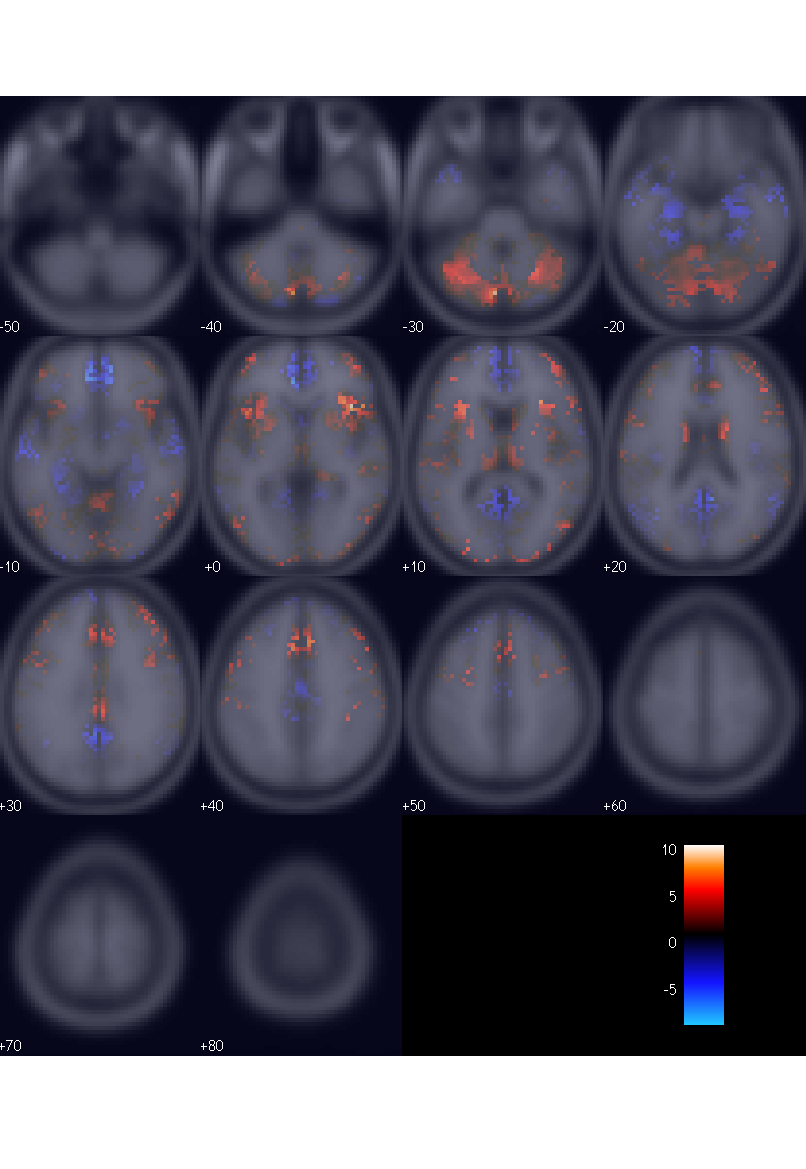
\includegraphics{f_map_gl_raw_t}
    \centering
	\caption{(Raw, that is unthresholded, $t$-values for all trials in the stimulus-response learning task (i.e. part 2), compared to the rest period,  overlaid onto the T1 MNI-352 template.   Each number is the height of the axial slice in MNI space.}
	\label{fig:glraw}
\end{figure}

\begin{figure}[tp]
	\fitfigure{f_map_gxl_p05}
    \centering
	\caption{Statistical parametric map for all trials in the stimulus-response learning task (i.e. part 2) examining the interaction between gains and losses.  \emph{Left} is a glass brain, showing all significant clusters mapped down to 3 two dimensional representations.  \emph{Right} is a set of axial slices highlighting strong areas of activity overlaid onto the T1 MNI-352 template.  $Z$ is the height of the axial slice in MNI space.}
	\label{fig:gxl}
\end{figure}

\subsection{Regions and models}
\label{sub:regoins}
\subsubsection{The right chunks}
\label{subsub:chunks}
Following whole-brain analysis, regions of interest were selected using two methods, that were later compared.  The first employed only regions from the Harvard-Oxford probabilistic anatomical atlas, using the 50\% cutoff \cite{Desikan:2006p9370}.  The second combined anatomical regions with functional clusters isolated using both sets of data collected during the second half of part 1 and from the reward-category localizer outlined above.  Analyses showed the clustered regions and entire anatomical regions displayed very similar model-fits.  So to limit the complexity of later analyses, and to increase power, functional analyses were dropped in favor of the larger anatomical regions.  Anatomical regions of interest were selected \emph{a priori} based on previous studies of reinforcement and category learning (see the \emph{Introduction for a review}).  Left and right subcortical regions of interest were the dorsal caudate, ventral striatum/nucleus accumbens, hippocampus, and amygdala.   Bilateral cortical areas were the middle frontal cortex (i.e. dorsal lateral PFC), superior frontal cortex (which contains ventral medial PFC), orbital frontal cortex, anterior and posterior cingulate (ACC and PCC for short).

% -- PROOFED ABOVE
\subsubsection{A Way To(o) Many}
\label{subsub:tomany}
In total there 6 models under evaluation -- the three kinds of similarity adjustment, (``none'', ``exp'', and ``gauss''), with two possible reward codes (``acc'' and ``gl'').  With the two terms of interest (i.e. value and the reward prediction error) that is 12 comparisons.  The are also a number of \emph{a priori} confounds to our signals of interest, the similarity metrics, the reward codes, and the grating parameters -- binging the total to 23.  However as the models are not nested\footnote{
    Often defined by whether or not tow models can be made identical by adding or subtracting parameters \cite{Forster:2000p9623}} and so are not amenable to $F$-tests, the common statistical way to compare fits.  Further complicating the issue is the fact that each of the models is covariate, if not collinear, with the others.  To top it off, none of the three are statistically independent; Reinforcement learning can viewed as a regression of the reward code onto behavioral choices (CITE).  All these factors combined would make statistical testing difficult.  But fortunately finding \emph{the} best model is not the goal.  

The latest recordings of phasic (i.e. reward prediction) activity in the VTA/SNc suggests a complicated reward and prediction error coding scheme (see p\pageref{subsub:expectations}), wherein several separate sets of calculations may be carried out independently \cite{Kim:2006p1063, Matsumoto:2009p7219, Smith:2011p8133}.  The observed BOLD signal is then an aggregate of these many activities, making it possible that more than one of the models under study is correct.  Under this constraint null hypothesis significance tests are not the right choice, model selection is.  Model selection is the process finding a \emph{family} of models/variates that best predict a given dataset \cite{Rao:2001p9457}, with most techniques trying to wisely balance parsimony with increasing fit (i.e. solving the bias versus variance dilemma \cite{Geman:1p9469}).  Unfortunately most model selection techniques require assumptions the models cannot meet (e.g. statistical independence).  The few that can tend to be complex recent statistical inventions.  And rather than navigate the those troubled and unproven waters, I took a simpler approach.  I examined each independently and ranked them.

A score (AIC, Akaike Information Criterion \cite{Akaike:1974p9530}) was assigned to each of the models/codes for every participant and region of interest.  Based on the average score across participants normalized based on the non-parametric (boxcar) model.  The absolute AIC score will vary by participant, but only the relative values are of interest.  Normalization based on the boxcar model, which serves somethings like a null hypothesis, provides a way to cast each participant's fits into relative terms suitable for averaging.  Using the normalized average score each model's performance was then ranked by subtracting each score from the best (lowest) score \cite{Anderson:2000p9475}. The normalized set was then transformed to Akaike Weights, a way to compare the conditional probabilities of each model being true \cite{Wagenmakers:2004p9472}.

\subsubsection{Information on Information}
\label{subsub:way}
AIC is a measure of loss; how much information is lost by substituting the model for the true distribution, i.e. the data.  The lower the AIC score, the better the model.  Unlike both the null hypothesis tests, and Bayesian measures, AIC based methods do not seek to find \emph{a} truth, but instead serve to rank models.  AIC offers then only relative insight, and is unable to make any claims about absolute significance.  Significance is a separate question, one I'll return to later.  Besides this limitation, AIC has some significant advantages. Five are reviewed below.

One, unlike maximum-likelihood AIC is designed to a be parsimonious score.  It penalizes for additional parameters.  It may therefore choose a worse model (as measured by likelihood or mean squared error) over a better but more complex one. This is the essence of Occam's razor\footnote{Famously and pithily expressed as, ``Entities are not to be multiplied beyond necessity''.}. 

Two, it fits with the process of science.  When designing an experiment it is rare that there are only two possible outcomes, instead typically there are several competing hypothesis, some of which may not be mutually exclusive.  AIC's focus on relative differences, and evidential weights, meshes perfectly with the reality of multiple working hypotheses \cite{Burnham:2004p9621}.

Three, truth can remain elusive.  A common alternative to AIC is BIC, the Bayesian Information Criterion.  Like AIC, it is derived from the log-likelihood of a model, however its derivation requires a rather strict (and often unrealistic) assumption -- that the true model is among the candidates \cite{Forster:2000p9623}.  And while it may be philosophically debatable whether any mathematical model can \emph{completely} describe reality, in this study it is a known fact that my models are incomplete.  The reinforcement learning literature contains several findings I (or anyone) can't yet account for (see the \emph{Introduction} for a review).  

Four, AIC values are easily interpretable once they're transformed to Akaike Likelihoods or Weights\footnote{
    Likelihood for model $k$ among $K$ working hypotheses/models is given by $L_k = e^{-0.5({AIC}_k - {min}_{K}{(AIC)})}$, which is then normalized, becoming an Akaike Weight by $w_k = L_k / \sum\limits_{k=1}^K L_k$ \cite{Burnham:2004p9621}.}.  The likelihood is simply the likelihood the model is correct (based on the information loss associated with it), while the Akaike Weights are just normalized likelihoods.  As the Weights sum to one, the conditional likelihood of one model compared to another is just the ratio of their weights \cite{Burnham:2004p9621}.  For example, if the conditional likelihood of model A over model B is $w_A/w_B$.  That is, the likelihoods and Akaike Weights are intrinsically measures of effect size \cite{Anderson:2000p9475,Forster:2000p9623}.  Despite the fact that it is often used to express the likelihood of correctly rejecting the null hypothesis, the $p$ value is not a measure of effect, as $p$ is contingent not just on effect size but on sample number.  
    
    Five, AIC has a history with models of categorization. \citeNP{McKinley:1996p9532,Maddox:2001p9533}, among several others, used AIC to compare behavioral results to several alternative models of categorization.  

\subsubsection{F-Them}
\label{subsub:F}
AIC ranks offer no information on significance, in the familiar null hypothesis sense, or on the absolute fit of the model.  I addressed both of these in a series of $F$-tests run prior to AIC analysis.  These (fixed-effect, across participant) ominbus tests asked whether the total set of regression parameters for each linear model (described below) could explain the BOLD time series better than chance, i.e could the null hypothesis (of 0) be rejected.  However in keeping with recommendations of \citeNP{Burnham:2004p9621, Forster:2000p9623}, who argue that as AIC and significance tests are so dissimilar that direct comparison/interaction between them them will be at best misleading, the models are not discarded based on significance.  Instead all models are retained, and later AIC ranked.  The $F$-tests are a separate measure whose results are integrated during interpretation, not during model selection/analysis.

\subsubsection{Code, BOLD, and Models.}
\label{sub:cmb}
A total of 23 models were compared for each of the 16 regions of interest for each of the 16 subjects, 5888 comparisons in total.  Each of the models is described below.  In general, a time-series (e.g the reward prediction error for each trial or the similarity for that trial's outcome) was convolved with a ``canonical''  haemodynamic response function, a mixture of gamma functions that serves as a parsimonious estimate of the (instantaneous) BOLD response \cite{Friston:1998p2022}, which was low-pass filtered matching the treatment of the BOLD data (p\pageref{subsub:preprocessed}).  Each convolved and filtered model was then regressed onto the BOLD response for each participant's region of interest, retaining all parameters and fit measures inside subject-level HDF5 files (\url{http://www.hdfgroup.org/HDF5/}).  

No available fMRI analysis package returns AIC scores (or measures that could be converted to such) and none allow for the efficient (i.e programmatic) analysis of many competing computational models. So I created a roi-focused fMRI data \emph{analysis} tool in Python (v2.7.1) to meet those two needs.  This module, simply named ``roi'', has since been release under the BSD license and is available for download at \url{https://github.com/andsoandso/roi}. It relies on the nibabel library to read the nifiti-1 files  (v1.2.0; \url{http://nipy.org/nibabel}), nitime for timeseries analysis, (v0.4; \url{http://nipy.sourceforge.net/nitime/}) Numpy for generic numerical work (v1.6.1; \url{http://numpy.scipy.org/}), with the GLS function from the scikits.statsmodels module handling the regerssions (v0.40; \url{http://statsmodels.sourceforge.net/}).  Model-to-BOLD fit parameters, as well as other useful metadata, was then extracted and stored in text files suitable for importing into R (v2.15.1; \url{http://www.r-project.org/}).  All plotting and model ranking (as well as the $F$-tests) were carried out in R.  For complete BSD licensed code see, \url{https://github.com/andsoandso/fmri/tree/master/catreward/roi/results}.

\subsubsection{Our Kinds of Models}
\label{subsub:ourkinds}
To simplify visualization and analysis, each of the models was classified into one of 5 families.  Family one, denoted ``boxcar'', was identical to that first used in the whole-brain analysis -- all trials versus the rest condition.  This is a univariate time-series that predicts no trial-specific effects; No matter the task the brain, thus the BOLD response, just flicks on then off.  It serves as a useful standard against which to compare the model-based regressors.  The next two families were controls (i.e. \emph{a priori} covariates), with the similarity metrics and grating parameters grouped into one family (``control\_similarity'') and the reward codes (both raw and similarity adjusted) into the other (``control\_reward'').  The fourth family was all the reward prediction errors (``rpe'').  The fifth was the value estimates (``value'').

\begin{center}
    \begin{longtable}{ | l | l | p{8cm} |}
    \caption{All models, their designations (Codes) and descriptions.}\\
    \hline
    Number & Code & Description \\ \hline
    1 & 0\_1 & The simplest model, a univariate analysis of all conditions. \\ \hline
    2 & acc & Behavioral accuracy. \\ \hline
    3 & acc\_exp & Behavioral accuracy, diminished by (exponential) similarity. \\ \hline
    4 & acc\_gauss & Behavioral accuracy, diminished by (gaussian) similarity. \\ \hline
    5 & gl & Gains and losses. \\ \hline 
    6 & gl\_exp & Gains and losses, diminished by (exponential) similarity. \\ \hline
    7 & gl\_gauss & Gains and losses, diminished by (gaussian) similarity. \\ \hline
    8 & rpe\_acc & Reward prediction error - derived from accuracy. \\ \hline
    9 & rpe\_acc\_exp & Reward prediction error - derived from accuracy diminished by (exponential) similarity. \\ \hline
    10 & rpe\_acc\_gauss & Reward prediction error - derived from accuracy diminished by (gaussian) similarity. \\ \hline
    11 & value\_acc & Value - derived from accuracy. \\ \hline
    12 & value\_acc\_exp & Value - derived from accuracy diminished by (exponential) similarity. \\ \hline
    13 & value\_acc\_guass & Value - derived from accuracy diminished by (gaussian) similarity. \\ \hline
    14 & rpe\_gl & Reward prediction error - derived from gains and loses. \\ \hline
    15 & rpe\_gl\_exp & Reward prediction error - derived from gains and losses diminished by (exponential) similarity. \\ \hline
    16 & rpe\_gl\_gauss & Reward prediction error - derived from gains and losses diminished by (gaussian) similarity. \\ \hline
    17 & value\_gl & Value - derived from gains and losses. \\ \hline
    18 & value\_gl\_exp & Value - derived from gains and losses diminished by (exponential) similarity. \\ \hline
    19 & value\_gl\_gauss & Value - derived from gains and losses diminished by (gaussian) similarity. \\ \hline 
    20 & exp & Outcome similarity (exponential). \\ \hline
    21 & gauss & Outcome similarity (gaussian). \\ \hline
    22 & angle & Grating angle parameter. \\ \hline
    23 &width & Grating width parameter. \\ \hline
    \end{longtable}
\end{center}


\subsection{Model Results}
\label{sub:modelresults}
\subsubsection{Under Cortical}
\label{subsub:belowctx}
Discuss the subcortical results first....

% -- Subcortical
\begin{figure}[tp]
	\fitfigure{f_meanpoint_bilatrun4_c_aic_Accumbens}
    \centering
    \caption{Nucleus Accumbens (left and right) -- Akaike Weights for all models.  Colors indicate model family (see p\pageref{sub:cmb} for details). Bars represent standard errors.}
	\label{fig:accumbens}
\end{figure}
\begin{figure}[tp]
	\fitfigure{f_plot_run4_c_fvalue_bilat_Accumbens}
    \centering
    \caption{Nucleus Accumbens (left and right) -- $F$-values for all models.  Significance is the $p <$ 0.05 level, trend is between $p <$ 0.05 and 0.10.  Colors indicate model family (see p\pageref{sub:cmb} for details).}
	\label{fig:fvalaccumbens}
\end{figure}


\begin{figure}[tp]
	\fitfigure{f_meanpoint_bilatrun4_c_aic_Amygdala}
    \centering
    \caption{Amygdala (left and right) -- Akaike Weights for all models.  Colors indicate model family (see p\pageref{sub:cmb} for details). Bars represent standard errors.}
	\label{fig:amygdala}
\end{figure}
\begin{figure}[tp]
	\fitfigure{f_plot_run4_c_fvalue_bilat_Amygdala}
    \centering
    \caption{Amygdala (left and right) -- $F$-values for all models.  Significance is the $p <$ 0.05 level, trend is between $p <$ 0.05 and 0.10.  Colors indicate model family (see p\pageref{sub:cmb} for details).}
	\label{fig:fvalamygdala}
\end{figure}


\begin{figure}[tp]
	\fitfigure{f_meanpoint_bilatrun4_c_aic_Caudate}
    \centering
    \caption{Dorsal Caudate (left and right) -- Akaike Weights for all models.  Colors indicate model family (see p\pageref{sub:cmb} for details). Bars represent standard errors.}
	\label{fig:caudate}
\end{figure}
\begin{figure}[tp]
	\fitfigure{f_plot_run4_c_fvalue_bilat_Caudate}
    \centering
    \caption{Dorsal Caudate (left and right) -- $F$-values for all models.  Significance is the $p <$ 0.05 level, trend is between $p <$ 0.05 and 0.10.  Colors indicate model family (see p\pageref{sub:cmb} for details).}
	\label{fig:fvalcaudate}
\end{figure}



\begin{figure}[tp]
	\fitfigure{f_meanpoint_bilatrun4_c_aic_Hippocampus}
    \centering
    \caption{Hippocampus (left and right) -- Akaike Weights for all models.  Colors indicate model family (see p\pageref{sub:cmb} for details). Bars represent standard errors.}
	\label{fig:hippocampus}
\end{figure}
\begin{figure}[tp]
	\fitfigure{f_plot_run4_c_fvalue_bilat_Hippocampus}
    \centering
    \caption{Hippocampus (left and right) -- $F$-values for all models.  Significance is the $p <$ 0.05 level, trend is between $p <$ 0.05 and 0.10.  Colors indicate model family (see p\pageref{sub:cmb} for details).}
	\label{fig:fvalhippocampus}
\end{figure}

\subsubsection{On that thinkin' sheet}
\label{subsub:onsheet}
Now discuss the cortical results....

\clearpage
% -- Cortex!
\begin{figure}[tp]
	\fitfigure{f_meanpoint_run4_c_aic_Cingulate_Gyrus_anterior_division}
    \centering
    \caption{Anterior Cingulate Gyrus -- Akaike Weights for all models.  Colors indicate model family (see p\pageref{sub:cmb} for details). Bars represent standard errors.}
	\label{fig:ant}
\end{figure}
\begin{figure}[tp]
	\fitfigure{f_plot_run4_c_fvalue_Cingulate_Gyrus_anterior_division}
    \centering
    \caption{Anterior Cingulate Gyrus -- $F$-values for all models.  Significance is the $p <$ 0.05 level, trend is between $p <$ 0.05 and 0.10.  Colors indicate model family (see p\pageref{sub:cmb} for details).}
	\label{fig:fvalant}
\end{figure}


\begin{figure}[tp]
	\fitfigure{f_meanpoint_run4_c_aic_Cingulate_Gyrus_posterior_division}
    \centering
    \caption{Posterior Cingulate Gyrus -- Akaike Weights for all models.  Colors indicate model family (see p\pageref{sub:cmb} for details). Bars represent standard errors.}
	\label{fig:post}
\end{figure}
\begin{figure}[tp]
	\fitfigure{f_plot_run4_c_fvalue_Cingulate_Gyrus_posterior_division}
    \centering
    \caption{Posterior Cingulate Gyrus -- $F$-values for all models.  Significance is the $p <$ 0.05 level, trend is between $p <$ 0.05 and 0.10.  Colors indicate model family (see p\pageref{sub:cmb} for details).}
	\label{fig:fvalpost}
\end{figure}


\begin{figure}[tp]
	\fitfigure{f_meanpoint_run4_c_aic_Frontal_Medial_Cortex}
    \centering
    \caption{Frontal (ventral) medial PFC -- Akaike Weights for all models.  Colors indicate model family (see p\pageref{sub:cmb} for details). Bars represent standard errors.}
	\label{fig:vmpfc}
\end{figure}
\begin{figure}[tp]
	\fitfigure{f_plot_run4_c_fvalue_Frontal_Medial_Cortex}
    \centering
    \caption{Frontal (ventral) medial PFC -- $F$-values for all models.  Significance is the $p <$ 0.05 level, trend is between $p <$ 0.05 and 0.10.  Colors indicate model family (see p\pageref{sub:cmb} for details).}
	\label{fig:fvalvmpfc}
\end{figure}


\begin{figure}[tp]
	\fitfigure{f_meanpoint_run4_c_aic_Frontal_Orbital_Cortex}
    \centering
    \caption{Orbital Frontal Cortex -- Akaike Weights for all models.  Colors indicate model family (see p\pageref{sub:cmb} for details). Bars represent standard errors.}
	\label{fig:ofc}
\end{figure}
\begin{figure}[tp]
	\fitfigure{f_plot_run4_c_fvalue_Frontal_Orbital_Cortex}
    \centering
    \caption{Orbital Frontal Cortex -- $F$-values for all models.  Significance is the $p <$ 0.05 level, trend is between $p <$ 0.05 and 0.10.  Colors indicate model family (see p\pageref{sub:cmb} for details).}
	\label{fig:fvalofc}
\end{figure}


\begin{figure}[tp]
    \fitfigure{f_meanpoint_run4_c_aic_Insular_Cortex}
    \centering
    \caption{Insula -- Akaike Weights for all models.  Colors indicate model family (see p\pageref{sub:cmb} for details). Bars represent standard errors.}
	\label{fig:insula}
\end{figure}
\begin{figure}[tp]
	\fitfigure{f_plot_run4_c_fvalue_Insular_Cortex}
    \centering
    \caption{Insula -- $F$-values for all models.  Significance is the $p <$ 0.05 level, trend is between $p <$ 0.05 and 0.10.  Colors indicate model family (see p\pageref{sub:cmb} for details).}
	\label{fig:fvalinsula}
\end{figure}


\begin{figure}[tp]
	\fitfigure{f_meanpoint_run4_c_aic_Middle_Frontal_Gyrus}
    \centering
    \caption{Middle Frontal (dorsal-lateral) PFC -- Akaike Weights for all models.  Colors indicate model family (see p\pageref{sub:cmb} for details). Bars represent standard errors.}
	\label{fig:dlpfc}
\end{figure}
\begin{figure}[tp]
	\fitfigure{f_plot_run4_c_fvalue_Middle_Frontal_Gyrus}
    \centering
    \caption{Middle Frontal (dorsal-lateral) PFC -- $F$-values for all models.  Significance is the $p <$ 0.05 level, trend is between $p <$ 0.05 and 0.10.  Colors indicate model family (see p\pageref{sub:cmb} for details).}
	\label{fig:fvaldlpfc}
\end{figure}

\clearpage
\newpage
\bibliography{bibmin}
%%%%%%%%%%%%%
\end{document}
%%%%%%%%%%%%%
